%% 
%% Copyright 2019-2021 Elsevier Ltd
%% 
%% This file is part of the 'CAS Bundle'.
%% --------------------------------------
%% 
%% It may be distributed under the conditions of the LaTeX Project Public
%% License, either version 1.2 of this license or (at your option) any
%% later version.  The latest version of this license is in
%%    http://www.latex-project.org/lppl.txt
%% and version 1.2 or later is part of all distributions of LaTeX
%% version 1999/12/01 or later.
%% 
%% The list of all files belonging to the 'CAS Bundle' is
%% given in the file `manifest.txt'.
%% 
%% Template article for cas-sc documentclass for 
%% single column output.

\documentclass[a4paper,fleqn]{cas-sc}

% If the frontmatter runs over more than one page 
% use the longmktitle option.

%\documentclass[a4paper,fleqn,longmktitle]{cas-sc}

%\usepackage[numbers]{natbib}
%\usepackage[authoryear]{natbib}
%\usepackage[authoryear,longnamesfirst]{natbib}
\usepackage[sort, numbers]{natbib}
% \usepackage[sorting=none]{biblatex}
\PassOptionsToPackage{table,dvipsnames,svgnames}{xcolor}
\usepackage{xcolor}
\usepackage{amssymb}% http://ctan.org/pkg/amssymb
\usepackage{mdframed}
\usepackage{times}
\usepackage{enumitem}
\usepackage[utf8]{inputenc}
\usepackage{geometry}
\usepackage{tcolorbox}
\usepackage{graphicx}
\usepackage{titlesec}
\usepackage{hyperref}
\usepackage{pifont}
\usepackage[utf8]{inputenc}
\usepackage{geometry}
\usepackage{tcolorbox}
\usepackage{graphicx}
\usepackage{titlesec}
\usepackage{enumitem}
\usepackage{amsmath,amsfonts}
\usepackage{algorithmic}
\usepackage{booktabs}
\usepackage{lipsum}
\usepackage{array}
\usepackage[caption=false,font=normalsize,labelfont=sf,textfont=sf]{subfig}
\usepackage{textcomp}
\usepackage{stfloats}
\usepackage{url}
\usepackage{multirow}
\usepackage{verbatim}
\usepackage{color}
\usepackage{tikz}   
\usepackage[toc,page]{appendix}
\usepackage{booktabs}
\usepackage{multirow}
\usepackage{graphicx}
\usepackage{caption}
% Custom section and subsection styles
\usepackage{setspace}  % 添加 setspace 包
% Custom tcolorbox styles
\tcbuselibrary{listingsutf8}
\tcbset{
  userstyle/.style={colback=blue!5!white, colframe=blue!75!black, sharp corners},
  defectstyle/.style={colback=green!5!white, colframe=green!75!black, sharp corners},
  gptstyle/.style={colback=red!5!white, colframe=red!75!black, sharp corners},
  boxsep=5pt, arc=4pt
}
% http://ctan.org/pkg/pifont
\newcommand{\cmark}{\ding{51}}%
\newcommand{\xmark}{\ding{55}}%
% algorithm package
\usepackage{epsfig}
\usepackage[linesnumbered,ruled,vlined,noline]{algorithm2e}
%\usepackage[sorting=none]{biblatex}
% For author et al. citation
% \usepackage[longnamesfirst, authoryear]{natbib}
\usepackage{multirow}
\usepackage{lineno}

\pagestyle{plain}

% Define et al.
\newcommand{\etal}{\textit{et al.}}

%\usepackage[linesnumbered,algoruled,boxed,lined]{algorithm2e}
%%%Author macros
\def\tsc#1{\csdef{#1}{\textsc{\lowercase{#1}}\xspace}}
\tsc{WGM}
\tsc{QE}
%%%

% Uncomment and use as if needed
%\newtheorem{theorem}{Theorem}
%\newtheorem{lemma}[theorem]{Lemma}
%\newdefinition{rmk}{Remark}
%\newproof{pf}{Proof}
%\newproof{pot}{Proof of Theorem \ref{thm}}
\begin{document}
% 调整行号间距,避免行号重叠
\renewcommand\linenumberfont{\normalfont\small}
\setlength\linenumbersep{10pt}
\linenumbers
\let\WriteBookmarks\relax
\def\floatpagepagefraction{1}
\def\textpagefraction{.001}
\pagestyle{plain}

\captionsetup[figure]{labelfont={bf},labelformat={default},labelsep=period,name={Fig.}}

% Short title
\shorttitle{DefectGPT: A LLM-based Integrated Building Digital Twin Information Retrieval-augmented Generation Framework and Its Application}    
% Short author
\shortauthors{Y. Huang~\etal}  
% Main title of the paper
\title [mode = title]{DefectGPT: A LLM-based Integrated Building Digital Twin Information Retrieval-augmented Generation Framework and Its Application}  
% Title footnote mark
% \tnotemark[1]

% Title footnote 1.
% \tnotetext[1]{This work was supported in part by the InnoHK of the Government of the Hong Kong Special Administrative Region via the Hong Kong Centre for Logistics Robotics and in part by the Research Grants Council of Hong Kong SAR (Grant Nos: 14217922, 14209623, 14209424 and 14200524).}

\author[1]{Yijun Huang}
\credit{Conceptualization, Data curation, Formal analysis, Investigation, Methodology, Software, Validation, Visualization, Writing - original draft}

\author[1]{Jihan Zhang}[type=editor,orcid=0009-0004-2773-1361]
\cormark[1]
\ead{1155139089@link.cuhk.edu.hk}
\credit{Investigation, Data curation, Visualization, Writing - review \& editing}

\author[1]{Qingxiang Li}
\credit{Investigation, Writing - review \& editing}

\author[1]{Xi Chen}[type=editor,orcid=0000-0003-2168-9057]
\cormark[1]
\ead{xichen002@cuhk.edu.hk}
\credit{Funding acquisition, Resources, Supervision, Writing - review \& editing}

\author[1]{Alan Lam}
\credit{Supervision, Writing - review \& editing}

\author[2,3,4]{Mirosław J. Skibniewski}
\credit{Supervision, Validation, Writing - review \& editing}

\author[1]{Ben M. Chen}
\credit{Funding acquisition, Resources, Supervision, Validation, Writing - review \& editing}

% Define corresponding authors
\cortext[cor1]{$\ast$Corresponding authors.}

% Author footnotes
% \fntext[fn1]{All authors contributed significantly to this work.}

\address[1]{Department of Mechanical and Automation Engineering, The Chinese University of Hong Kong, Shatin, N.T., Hong Kong, China}
\address[2]{Department of Civil and Environmental Engineering, University of Maryland, College Park, MD 20742, USA}
\address[3]{Polish Academy of Sciences Institute of Theoretical Informatics, Gliwice, Poland}
\address[4]{Chaoyang University of Technology, Taichung, Taiwan}

% Here goes the abstract
\begin{abstract}
The emergence of Large Language Models (LLMs) provides previously unattainable cognitive capabilities for solving complex problems. However, when applying them to high-risk, dynamic physical world decision-making, a fundamental ``cognitive-physical gap'' exists. This gap manifests as three core technical challenges: the ``reality grounding'' problem where LLMs struggle to accurately understand multimodal, structured data from physical systems; the ``model utilization'' problem where they cannot effectively invoke and orchestrate complex physical simulation models; and the ``safe execution'' problem where they fail to coordinate their slow reasoning with the rapid, safe response requirements of the physical world.

To systematically address these challenges, a doctoral research plan has been formulated, centered on conceptualizing and designing a new Agent architecture named CORTEX. The theoretical foundation of this work is a novel ``three-tier digital twin decision framework.'' This framework categorizes physical decision tasks by complexity evolution into three levels: L1-Descriptive Twins (for diagnostic decisions), L2-Predictive Twins (for strategic decisions), and L3-Interactive Twins (for action-oriented decisions). This framework not only provides logical justification for CORTEX architecture design but also constructs a standardized ``capability testing ground'' for subsequent empirical evaluation.

The CORTEX architecture directly responds to the three challenges through deep extensions of existing paradigms. Its ``Perception Module'' employs a novel Digital Twin Retrieval-Augmented Generation (DT-RAG) mechanism to address reality grounding; its ``Reasoning Module'' encapsulates complex physical models as LLM-callable tools to address model utilization; and its ``Action Module'' designs a ``slow-fast dual-loop'' safety coordinator to address safe execution.

The effectiveness of this architecture will be rigorously evaluated through a series of representative cases. The evaluation centers on quantifying a metric called ``Cognitive Gain'' to measure the performance improvement CORTEX brings compared to the best traditional methods in the field. Three case studies map to L1, L2, and L3 levels respectively: structural health diagnosis of buildings at L1 level, cancer treatment strategy planning based on tumor microenvironment twins at L2 level, and autonomous UAV exploration in unknown environments at L3 level.

Ultimately, this doctoral research aims to deliver a thoroughly validated, scalable architectural blueprint, laying the foundation for future development of powerful next-generation artificial intelligence systems capable of advanced reasoning and reliable action in complex, dynamic physical worlds.
\end{abstract}

% Research highlights
\nolinenumbers
\begin{highlights}
\item Building inspection framework combining Digital Twin (DT) technology, multi-source data fusion, and Large Language Models (LLMs)
\item Domain-specific Retrieval-Augmented Generation (RAG) system for building defect management with context-aware information retrieval
\item Automated defect knowledge engine with dynamic updates from multi-source inspection data streams
\item Natural language query interface enabling contextual analysis of defect evolution and maintenance recommendations
\item Validation through real-world deployment on high-rise building inspection with significant improvements in defect analysis efficiency
\end{highlights}
\linenumbers

% Keywords
% Each keyword is separated by \sep
\begin{keywords}
Building Defect Management \sep Large Language Models (LLMs) \sep Retrieval-Augmented Generation (RAG) \sep Digital Twin (DT) \sep Building Information Model (BIM) \sep Geographic Information System (GIS)
\end{keywords}

\maketitle
% Main text

\section{Introduction}

In the contemporary process of urbanization, buildings serve as the core carriers of human activity, with their safety and functionality directly related to social stability and development. However, as time progresses, buildings inevitably face issues of aging and wear. According to the latest statistical data, over 50\% of private residences experience varying degrees of structural problems after 30 years of use \cite{spencer2019advances}. These issues range from surface cracks to severe structural defects, not only affecting the aesthetics and comfort of buildings but more seriously, potentially endangering the lives and property of users \cite{zhang2023automated}.

Traditional building defect management has evolved through different data governance paradigms. Document-based approaches, relying on inspection reports, maintenance logs, and repair records, suffer from unstructured information organization and limited searchability. Model-based methods, leveraging Building Information Models (BIMs) and Geographic Information Systems (GIS), provide better structure but lack flexibility in handling dynamic defect information and complex semantic relationships \cite{li2024single}. Both approaches struggle with the temporal nature of defect evolution and the complex interdependencies between different building components.

The unique characteristics of building defects pose specific challenges for information management. Defects are inherently dynamic, evolving over time with varying progression patterns. They exhibit complex spatial-temporal relationships, where one defect may influence or indicate potential issues in other building components. Traditional defect modeling approaches often fail to capture these dynamic relationships and evolution patterns effectively \cite{wang2023augmented}. Furthermore, the interpretation and assessment of defects require extensive domain expertise, making it difficult to standardize the evaluation process.

With the advent of Industry 4.0, emerging technologies have provided new possibilities for addressing these challenges. Unmanned Aerial Vehicle (UAV) technology, with its flexibility and efficiency, can rapidly acquire high-resolution image data of building surfaces, greatly improving the efficiency and comprehensiveness of data collection \cite{mohammadi2023integration}. Digital Twin (DT) technology, by creating virtual models of buildings, has realized real-time mapping and interaction between the physical and digital worlds, providing powerful tools for the visualization and predictive analysis of building defects \cite{chen2023improving}.

The maturation of Large Language Models (LLMs) offers a new paradigm for defect information management. These models excel at understanding complex semantic relationships and can process both structured and unstructured data, making them particularly suitable for building defect management \cite{gao2023survey}. However, the direct application of LLMs faces challenges in domain-specific knowledge integration and real-time information updating.

To address these limitations, this study proposes an intelligent building defect management framework based on agentic Retrieval-Augmented Generation (RAG) technology. The framework introduces a novel defect modeling approach that captures the dynamic nature and complex relationships of building defects. By integrating this domain-specific defect model with LLM capabilities through an agent-based architecture, the system can provide context-aware, expertise-driven defect analysis and management \cite{ding2024survey}.

The main contributions of this research include:

\begin{enumerate}
\item \textbf{An innovative intelligent building defect information retrieval and generation framework}: We propose a comprehensive framework that seamlessly combines UAV data acquisition, DT technology, and LLMs. In this framework, LLMs serve as the central component, enhancing the understanding and analysis of building defects by processing complex semantic information extracted from multi-source data.

\item \textbf{Development of a domain-specific modeling approach using LLMs}: We introduce an innovative method for modeling building defects that leverages the capabilities of LLMs. This approach enables accurate interpretation of complex and dynamic defect patterns by capturing the nuanced relationships and contextual dependencies inherent in building defect data. It empowers the system to provide expert-level analysis and predictions tailored to the specific characteristics of the building domain.

\item \textbf{Integration of RAG techniques to enhance LLM performance}: To address the limitations of LLMs in domain knowledge integration and real-time information updating, we incorporate RAG into our framework. This integration enhances the system's ability to retrieve relevant domain-specific knowledge efficiently and generate accurate, context-aware responses. It significantly improves the system's knowledge retrieval accuracy and information generation reliability, ensuring that analyses and recommendations are both up-to-date and grounded in the most pertinent information available.
\end{enumerate}

These contributions collectively advance the field of intelligent building defect management by providing a flexible, efficient, and reliable approach that leverages state-of-the-art artificial intelligence technologies. By focusing on LLMs and enhancing their capabilities through RAG, our framework addresses critical challenges in processing complex, dynamic, and domain-specific information inherent in modern building defect analysis.

To validate the effectiveness and feasibility of the proposed framework, we selected a high-rise building over 100m tall for a year-long defect monitoring and management study \cite{zhang2023automated}. Through this practical case, we comprehensively evaluated the system's performance on multiple indicators such as defect detection accuracy, response time, and user satisfaction, and conducted detailed comparisons with traditional methods.

The subsequent sections of this paper are arranged as follows: Section 2 provides a detailed review of related work, including the application of DT technology in building management, the application of deep learning in data analysis, information retrieval and generation technologies, and multi-source data integration technologies. We systematically analyze the advantages and limitations of existing methods, providing a theoretical foundation for the innovative points of this research. Section 3 delves into the theoretical framework of our proposed intelligent defect data analysis agent. We describe in detail each component of the framework from multiple perspectives such as system architecture, data flow, and algorithm design, with a focus on explaining the application of RAG technology and LLMs. Section 4 validates the effectiveness of our proposed framework through the aforementioned high-rise building case, including detailed experimental design, result analysis, and performance evaluation. Finally, Section 5 summarizes the main findings and contributions of this research, discusses the limitations of the current method, and looks ahead to future research directions.


\section{Literature review}
\label{sec: comparison_results}

\subsection{UAV-based building inspection methods}

The integration of UAVs into building inspection marks a significant shift from traditional, labor-intensive, and hazardous methods to more efficient, safer, and cost-effective approaches \cite{zhang2022integrating}. Studies have reported time savings of 60--70\% and around 40\% increases in defect detection accuracy compared to conventional techniques \cite{falorca2021facade, ruiz2021unmanned}. Modern UAV-based systems leverage multiple sensors, such as thermal, multispectral, and LiDAR, enabling comprehensive assessments that identify both visible defects (e.g., cracks, spalling) and hidden structural issues beneath the surface \cite{kim2017concrete, jiang2020real}. This multi-sensor capability is particularly valuable for large-scale building portfolios, post-disaster damage evaluation, and hard-to-reach areas like high-rise façades and complex roof structures.

Despite these advances, several challenges persist. The substantial volume of data generated by UAV surveys often poses difficulties in efficient storage, organization, and analysis \cite{chen2021geo}. Equally challenging is the precise localization of detected defects within the broader building model. To address these issues, recent studies have examined the integration of UAV-acquired data with BIM systems, facilitating more accurate flight path planning, contextualized defect documentation, and streamlined data management workflows \cite{tan2021automatic, liu2021integrating}.

Furthermore, autonomous UAV inspection has gained traction, incorporating advanced algorithms for obstacle avoidance and optimized flight trajectories. This reduces operator workload and ensures consistent coverage, while onboard machine learning models enable real-time defect detection and classification \cite{ribeiro2020remote, tan2021automatic}. Future research directions include enhancing sensor modalities, refining data processing algorithms, and exploring cloud or edge computing solutions to manage large datasets more efficiently \cite{nepal2021towards}. Ultimately, combining UAV technology with BIM and AI-driven analytics paves the way for more integrated, scalable, and intelligent building inspection solutions.

\subsection{DT Technologies in building management}
DT technology has revolutionized building management by providing real-time, data-driven representations of physical structures. This technological advancement has enabled more efficient inspection processes, improved maintenance planning, and enhanced decision-making capabilities. The integration of various DT technologies, particularly BIM and GIS, has created comprehensive platforms for building lifecycle management \cite{zhang2022integrating}.

\subsubsection{BIM-based approaches}

BIM serves as a fundamental component of DT implementation in building management. The application of BIM for defect documentation has shown significant advantages in maintaining comprehensive building condition records. Bruno et al. \cite{bruno2018historic} demonstrated how BIM can effectively capture and store detailed information about building defects, including their location, severity, and temporal evolution. This capability has proven particularly valuable for tracking maintenance history and planning future interventions.

The integration of BIM with maintenance systems represents another significant advancement in building management. Ismail \cite{ismail2021how} developed a framework that connects BIM models with maintenance management systems, enabling automated scheduling of inspections and repairs based on documented defect patterns. This integration has shown potential for reducing maintenance response times by up to 40\% while improving the accuracy of intervention planning.

Semantic modeling capabilities within BIM environments have enhanced our ability to understand and analyze building defects. Hamdan et al. \cite{hamdan2021semantic} proposed a semantic modeling approach that enables automated interpretation of structural damage within BIM models. This advancement allows for more sophisticated analysis of defect patterns and their potential implications for building performance. However, limitations in real-time updates remain a significant challenge, particularly when dealing with rapidly evolving defect conditions or emergency situations.

\subsubsection{GIS-based approaches}

Geographic Information Systems have emerged as powerful tools for spatial analysis and visualization in building management. Tsilimantou et al. \cite{tsilimantou2020gis} demonstrated the effectiveness of GIS in managing building inspection data across multiple spatial scales. Their research showed how GIS can facilitate the analysis of defect patterns in large portfolios of buildings, allowing a better understanding of environmental and location-based factors that affect building deterioration.

Multi-scale defect mapping through GIS has provided new insights into building performance patterns. Chen et al. \cite{chen2021geo} developed a GIS-based approach for managing UAV-captured inspection images, enabling precise localization of defects within building facades. This integration of spatial data with defect documentation has improved our ability to identify and analyze patterns of building deterioration across different scales.

Environmental context integration represents a key advantage of GIS-based approaches. Nepal et al. \cite{nepal2021towards} showed how GIS can help correlate building defects with environmental factors, enabling a better understanding of external influences on building deterioration. However, challenges remain in achieving sufficient detail for precise inspection documentation, particularly when dealing with fine-scale defects or complex structural issues.

\subsubsection{Other approaches}

Beyond BIM and GIS, several management platforms have emerged to enhance building inspection and maintenance capabilities. AR-based visualization platforms represent a significant advancement in this domain. May et al. \cite{may2022identification} demonstrated the potential of BIM-based AR platforms for defect management inspections, which enabled more intuitive visualization of building information and improved inspection accuracy compared to traditional paper-based methods. Their BIM-ARDM system integrated real-time 3D visualization with tablet-based data collection interfaces, showing significant improvements in task performance, mental workload, completion time, and defect identification accuracy.

The development of AR-based platforms has evolved significantly over the past decade. Early implementations by Shin and Dunston \cite{shin2009framework} identified eight key construction tasks where AR could provide benefits, including layout, excavation, positioning, inspection, coordination, supervision, commenting, and strategizing. Recent advancements have led to more sophisticated systems, such as García-Pereira et al.'s \cite{garcia2020annotation} annotation-based inspection tool that achieved excellent usability rankings and demonstrated potential for reducing inspection time and improving documentation processes.

Web-based management platforms have emerged as another important approach. Ma et al. \cite{ma2021single} developed a tablet-based quality management inspection system that integrated BIM models and indoor positioning, demonstrating significant improvements in inspection efficiency. Their system reduced the overall inspection process time by approximately 50\% compared to traditional methods, particularly in aspects such as planning, result summarization, and communication. Park et al. \cite{park2013framework} proposed a conceptual proactive construction defect management framework that integrated multiple approaches to improve upon conventional manual inspection processes.

Intelligent decision support platforms represent another significant development in building management. These systems leverage advanced data analysis and artificial intelligence to enhance decision-making processes. Zhou et al. \cite{zhou2019development} developed an AR system for tunnel construction inspection that demonstrated superior performance in diagnosing segment displacement compared to conventional methods. Similarly, Kwon et al. \cite{kwon2019defect} presented both remote and on-site AR-based prototypes for defect management inspections, incorporating image-matching techniques to overcome traditional manual inspection limitations.

The integration of various visualization techniques has also proven valuable in building management platforms. Portalés et al. \cite{portales2018digital} developed an AR tablet-based inspection tool that incorporated advanced visualizations for prefabricated buildings, demonstrating the potential of combining different visualization approaches in a single platform. Feng et al. \cite{feng2020visualization} utilized head-mounted displays to develop an AR-based inspection tool that superimposed BIM models onto physical construction sites, further advancing the field of visualization in building management.

The evolution of these management platforms - BIM, GIS, AR-based, web-based, and intelligent decision support systems - represents significant progress toward more comprehensive building management solutions. While each platform brings unique strengths, future developments will likely focus on improving interoperability between these approaches. The potential for combining the spatial analysis capabilities of GIS, the detailed building information from BIM, and the intuitive visualization of AR platforms shows promise in creating more effective building management solutions. However, challenges remain in achieving seamless integration between different platforms and ensuring consistent data quality across various systems \cite{hola2015identification}. These challenges include issues related to data exchange standards, hardware limitations, and the need for improved tracking accuracy in AR implementations \cite{may2022identification}.

This diverse ecosystem of management platforms reflects the industry's movement toward more sophisticated and integrated approaches to building management. Each platform type offers distinct advantages: AR-based platforms excel in visualization and real-time inspection support, web-based platforms facilitate improved data management and communication, and intelligent decision support systems enhance analytical capabilities. The continued development and integration of these various approaches suggest a future where building management becomes increasingly efficient, accurate, and comprehensive.

\subsection{Large language models in building information management}

The integration of LLMs into building information management represents a transformative advancement in automated compliance checking and information processing. Recent developments in LLMs have demonstrated remarkable capabilities in understanding and processing complex building regulations and technical documentation \cite{chen2023automated}. Through extensive pre-training on diverse corpora, these models have shown exceptional ability to comprehend complex technical language and contextual relationships within building regulations \cite{brown2020language}, effectively processing various types of construction documentation, including inspection reports, maintenance records, and technical specifications, and converting unstructured text into structured, actionable information \cite{gao2023survey}.

The application of LLMs in automated compliance checking has been significantly enhanced through RAG approaches \cite{lewis2020retrieval, fan2023retrieval}. This integration enables more precise and reliable processing of domain-specific information by combining the general knowledge embedded in pre-trained models with specialized construction knowledge \cite{fan2023retrieval}. The effectiveness of RAG systems in construction applications has been demonstrated by several recent studies \cite{asai2023self, wang2023augmented}, showing particular promise in handling complex regulatory texts and technical specifications with high accuracy and consistency.

The effectiveness of LLMs in handling technical documentation has been significantly improved through their integration with domain ontologies and BIM systems \cite{bruno2018historic, ismail2021how}. Hamdan et al. \cite{hamdan2021semantic} demonstrated how combining LLMs with domain-specific knowledge models can improve the accuracy of information extraction from building regulations, achieving significant improvements in both precision and recall compared to traditional methods. This integration has enabled more sophisticated approaches to compliance verification, as shown by Tsilimantou et al. \cite{tsilimantou2020gis}, who developed methods to automate the inspection data collection process while maintaining high accuracy in regulatory interpretation and compliance assessment.

Recent innovations have focused on developing comprehensive frameworks that combine LLMs with other advanced technologies \cite{zhang2022integrating, chen2021geo}. Nepal et al. \cite{nepal2021towards} proposed an innovative approach combining LLMs with deep learning models and ontology knowledge models for automated compliance checking. Their system demonstrated superior performance in processing complex regulatory texts with nested clauses and conditional statements, extracting structured information from unstructured building codes, and generating accurate compliance reports with detailed explanations. This approach represents a significant advancement over traditional rule-based systems \cite{ribeiro2020remote, tan2021automatic}, offering more flexible and adaptive solutions for building information management.

% \begin{figure}[h]
%     \centering
%     \includegraphics[width=1\linewidth]{output-3.png}
%     \caption{Defect-Based Maintenance Decision Improvement showing comparative analysis across different maintenance parameters}
%     \label{fig:maintenance-improvement}
% \end{figure}

Despite these advances, several significant challenges remain in the application of LLMs to building information management \cite{li2023explaining, meng2023self}. Data privacy and security concerns in handling sensitive building information when using cloud-based LLM services present significant challenges \cite{mohammadi2023integration}. Chen et al. \cite{chen2023improving} explored the complexities of integrating LLMs with existing BIM systems and workflows, while Li et al. \cite{li2024single} addressed the challenges of ensuring consistency and accuracy in LLM-generated outputs for construction applications. These challenges continue to drive research and development in the field, with future developments likely focusing on enhancing the interpretability of LLM decisions and improving domain-specific training approaches \cite{fan2023retrieval}.

The evolution of LLMs in building information management represents a significant step toward more efficient and effective automated compliance checking systems \cite{fan2023retrieval}. While current implementations have demonstrated substantial improvements in processing efficiency and accuracy, continued research is needed to address existing limitations and expand system capabilities \cite{borgeaud2022improving, izacard2021leveraging}. The integration of LLMs with other emerging technologies, particularly BIM and artificial intelligence, shows promise in creating more comprehensive and automated building inspection solutions. As these technologies continue to mature and become more specialized for construction-related applications, their potential to revolutionize building information management grows, offering increasingly sophisticated solutions for the challenges faced by the construction industry.

\section{Proposed framework}

We propose a comprehensive framework, DefectGPT, that integrates DT technology, RAG, and LLMs to address the challenges of modern building inspection and defect management. As illustrated in Fig.~\ref{fig:framework}, this framework is designed to provide precise, scalable, and context-aware solutions for identifying, monitoring, and managing structural anomalies, leveraging advanced spatial data processing, semantic enrichment, and intelligent decision-making.


\begin{figure}
\centering
\includegraphics[width=0.8\linewidth]{Overall_Framework.png}
\caption{The overall framework of DefectGPT showing the integration of three core components}
\label{fig:framework}
\end{figure}


The framework depicted in Fig.~\ref{fig:framework} comprises six interconnected components organized around a central processing core. The Context-Aware Retrieval Engine implements sophisticated algorithms for hybrid knowledge access, enabling intelligent information retrieval that considers not only explicit queries but also the implicit contextual parameters of building components, environmental factors, and historical maintenance records. This engine works in concert with the Digital Twin Technology component, which establishes a bidirectional bridge between physical and digital realms, maintaining high-fidelity virtual representations that are continuously synchronized with their physical counterparts. The Hierarchical Knowledge Base constitutes the third critical component, storing domain expertise and historical records in a taxonomically structured format that facilitates efficient retrieval and inference according to established building engineering principles and industry standards.

Complementing these components, the Multi-Source Data Integration module harmonizes heterogeneous data streams from various inspection methodologies, sensor systems, and documentation repositories to create a unified and comprehensive representation of building conditions. This integrated data undergoes further processing through the Semantic Enrichment Processor, which augments raw defect information with contextual metadata, significantly enhancing interpretability through semantic annotations that describe relationships, classifications, and domain-specific attributes. The final component, the Spatial Registration Engine, implements advanced algorithms to map detected defects onto georeferenced building components, enabling precise localization and temporal tracking of structural anomalies within the three-dimensional architectural model. The central integration hub represented in Fig.~\ref{fig:framework} functions as the nexus for alert management, notification prioritization, and critical information synthesis based on severity metrics and contextual relevance.

This architectural framework transcends the limitations of conventional building inspection methodologies by facilitating: (1) seamless integration of heterogeneous data sources across multiple modalities and formats, (2) precise spatial registration of defect information within complex three-dimensional building models, (3) context-aware knowledge retrieval that considers both explicit and implicit query parameters, (4) automated semantic enrichment through domain-specific ontologies, and (5) intelligent decision support through advanced computational modeling techniques. 

The subsequent sections examine these components in detail, beginning with DT Modeling, which serves as the foundational infrastructure for spatial representation and defect contextualization. We then analyze the RAG-enhanced knowledge management system that enables sophisticated information retrieval and organizational capabilities. Finally, we present the LLM-based intelligence layer that transforms structured knowledge repositories into actionable insights and evidence-based recommendations for building maintenance planning and management.

\subsection{DT Modeling}
Building upon our previous work in GeoBIM-assisted registration for building façade defects~\cite{zhang2024automated}, we present a comprehensive BIM+GIS-based DT modeling framework implementing a three-layer architecture comprising the \textbf{Data Layer}, the \textbf{DT Layer}, and the newly introduced \textbf{Decision Layer}. This structure enables sophisticated data management and real-time synchronization between physical buildings and their digital counterparts, facilitating advanced monitoring, analysis, and decision-making in building defect management~\cite{mill2013combined,pantoja2023damage}.

As shown in Fig.~\ref{fig:dt-framework}, the \textbf{Data Layer} incorporates three primary components: GeoBIM modeling, defect modeling, and expert knowledge integration. The GeoBIM modeling component combines multiple data sources, including 3D mesh models, BIM models, GIS information, and geo-AI knowledge bases, following our previously established integration approach~\cite{zhang2024automated} and building upon frameworks proposed by~\cite{xia2022study} and~\cite{chen2023improving}. The defect modeling component processes aerial photographs of building facades, employing detection algorithms to identify RGB defects, infrared anomalies, and defect classifications~\cite{shi2020review,hosamo2022digital}. Furthermore, it performs precise defect localization, determining global positions, local coordinates, and characteristic defect data features. Expert knowledge integration leverages inspection reports, technical standards, legal frameworks, and defect manuals to enrich the defect data with domain-specific insights.

The \textbf{DT Layer} serves as the core of the digital representation, implementing three distinct data carriers to manage and organize the diverse information streams, extending the approaches presented in~\cite{jati2021uav,fitkau2024ontology}. Spatial information carriers handle formats such as IFC, RVT, and KML, ensuring proper management of spatial data and geometric relationships in line with~\cite{li2024single,zeng2024conse}. Additionally, defect data schemas (XML, JSON, CSV, database) and domain knowledge repositories (PDF, DOCX, Markdown) provide standardized storage formats, ensuring seamless compatibility with the retrieval workflows. The DT Layer maintains temporal records of defect evolution and allows real-time updates from periodic UAV surveys and sensor monitoring~\cite{tan2022mapping,zhang2023automated}.

The \textbf{Decision Layer} leverages retrieval augmented generation (RAG) and large language model (LLM) techniques for advanced reasoning and human-in-the-loop decision-making. By storing vector embeddings in databases, retrieving and reranking relevant chunks of domain-specific information, and routing user queries through AI-driven modules, this layer provides actionable insights in building defect management. Users can query the system (e.g., "Illustrate the distribution of cracks…"), and the Decision Layer integrates data streams from the DT, domain knowledge repositories, and spatial information carriers to generate intuitive visualizations, predictive maintenance insights, and other decision supports.

\begin{figure*}[t!]
    \centering
    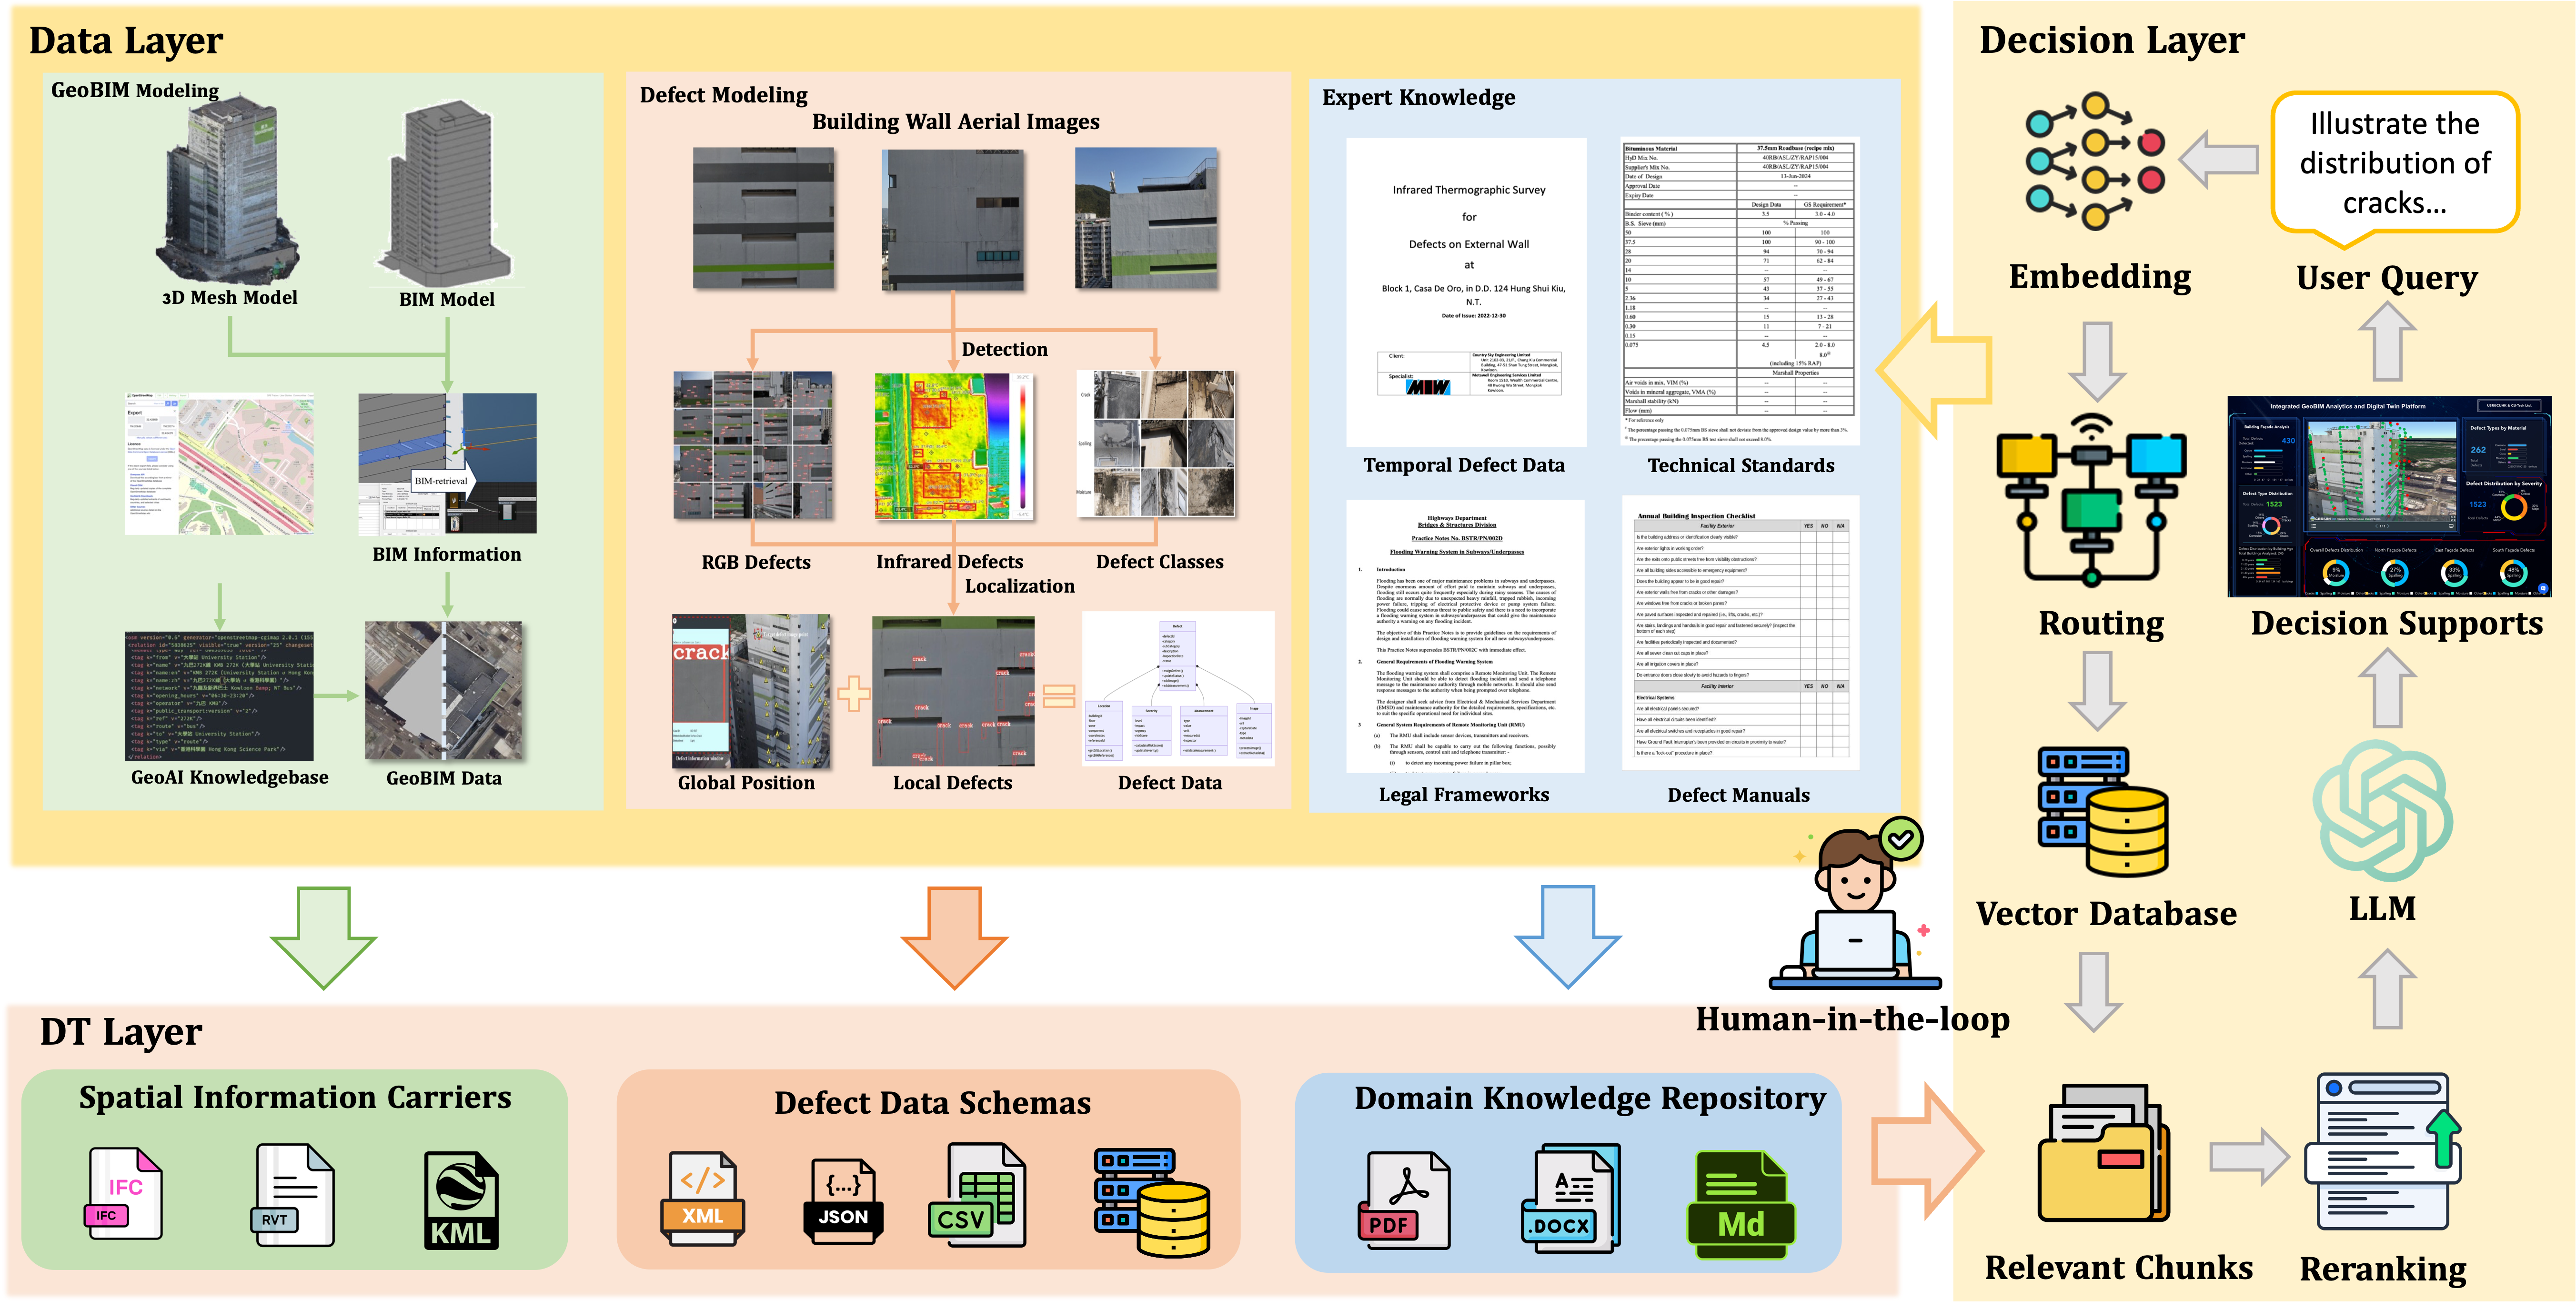
\includegraphics[width=1\linewidth]{dt-framework.png}
    \caption{A comprehensive DT architecture for building defect management, illustrating the three-layer structure: (1) Data Layer, (2) DT Layer, and (3) Decision Layer.}
    \label{fig:dt-framework}
\end{figure*}

Defect localization begins with UAV-based inspections capturing high-resolution images of building facades. Using RTK (Real-Time Kinematic) positioning, the UAV's pose is accurately determined, ensuring precise alignment between captured images and the 3D BIM model. Detected defects (RGB or infrared) are bound with bounding boxes and classifications, subsequently mapped from 2D image coordinates onto the 3D BIM model. The coordinate transformation involves depth and pose estimation, followed by tangential vector adjustments to align detected defects with facade surfaces.

\begin{algorithm}[t!]
\caption{Defect global localization}
\label{al:1}
\begin{algorithmic}[1]
\REQUIRE Geographical coordinates of image $P_{i}^{g}(lon_{i}, lat_{i}, alt_{i})$; Distance to the wall $d_{wall}$; Projection vector $\vec{n}$
\ENSURE Global location of defect $d_{i,j}$: $g(i,j)(lng_{i,j}, lat_{i,j}, alt_{i,j})$
\STATE Initialize array of detected images $i$
\STATE \textbf{for} $t = 1$ to $i_{\max}$ \textbf{do}
\STATE \hspace{1em}Project from image localization $P_{i}^{g}$ to the corresponding point on the wall
\STATE \hspace{1em}Given $\vec{n} = (\alpha_{i}, \beta_{i}, \gamma_{i})$
\STATE \hspace{1em}$P^{g\ast}_{i} = P^{g}_{i} + d_{wall} * \vec{n}$
\STATE \hspace{1em}\textbf{for} $j = 1$ to $j_{\max}$ \textbf{do}
\STATE \hspace{2em}$L_{D}(i) = 2d_{wall} \tan{\frac{FOV}{2}}$
\STATE \hspace{2em}$\vec{L}(i,j) = L_{D}(i) \cdot \frac{l(i,j)}{l_{D}(i)}$
\STATE \hspace{2em}$g(i,j) = P^{g\ast}_{i} + \vec{L}(i,j)$
\STATE \hspace{2em}$T \gets \sqrt{ \bigl(\tfrac{0.5}{unit_{lng}}\bigr)^2 + \bigl(\tfrac{0.5}{unit_{lat}}\bigr)^2 }$
\STATE \hspace{2em}\textbf{for} $k = 1$ to $i-1$ \textbf{do}
\STATE \hspace{3em}\textbf{for} $t' = 1$ to $j_{\max}-1$ \textbf{do}
\STATE \hspace{4em}\textbf{if} $\sqrt{(g(k,t') - g(i,j))^2} > T$ \textbf{then}
\STATE \hspace{5em}Register new defect $g(i,j)$
\RETURN $g(i,j)(lng_{i,j}, lat_{i,j}, alt_{i,j})$
\end{algorithmic}
\end{algorithm}

Through the integration of GIS and BIM data, the DT environment unifies defect information with broader spatial context~\cite{chen2023gis}. The BIM model offers geometric and semantic data on structural elements, while GIS data provides real-world context, enabling geo-referencing and scalable defect tracking. The DT architecture also accommodates incremental updating approaches, allowing new data from UAV surveys and sensors to be injected without reconstructing the entire model~\cite{zhang2024automated}. By preparing structured, enriched, and contextually relevant data streams, this DT modeling stage ensures the \textbf{Decision Layer} has access to consistent and comprehensive information for retrieval, query, and generation tasks. The combination of spatial, semantic, and domain knowledge fosters advanced decision-making and efficient defect management processes.


\subsection{LLM-based intelligence layer}
The intelligence layer represents a critical component of our framework, leveraging LLMs to provide sophisticated analysis and decision support capabilities for building defect management. Unlike traditional rule-based systems, our approach integrates advanced natural language processing capabilities with domain-specific knowledge, enabling intelligent interpretation of building inspection data and generation of actionable insights. The core architecture combines pre-trained LLMs with specialized fine-tuning mechanisms that incorporate building engineering expertise, defect pattern recognition, and maintenance protocols.

As illustrated in Fig.~\ref{fig:llm_architecture}, our system architecture implements a comprehensive pipeline consisting of three primary stages: indexing, retrieval, and generation. The indexing pipeline begins with raw defect data processing, where inspection reports, sensor readings, and maintenance records are systematically chunked and transformed into high-dimensional embeddings. These embeddings, generated through the text-embedding-3-large model, capture the semantic relationships within technical documentation while preserving domain-specific nuances. The vector store, implemented using FAISS with IVF-PQ compression, enables efficient similarity search across millions of document fragments.

The retrieval engine employs a dual-path architecture that enhances result comprehensiveness and reliability. The primary path performs vector-based similarity search against the indexed document store, identifying the most relevant historical cases and technical specifications. Concurrently, the secondary path conducts targeted web searches within authorized external sources, particularly for regulatory updates and emerging repair techniques. The context integration module then merges these results using a sophisticated scoring function:

\begin{equation}
S_{relevance} = \alpha \cdot sim(q, d) + \beta \cdot freshness(d) + \gamma \cdot authority(d)
\label{eq:relevance}
\end{equation}

where $sim(q, d)$ represents the cosine similarity between query and document embeddings, $freshness(d)$ accounts for temporal relevance, and $authority(d)$ weighs source credibility. The parameters $\alpha$, $\beta$, and $\gamma$ are dynamically tuned through continuous validation against expert assessments.

The generation module, powered by a domain-fine-tuned GPT-4 model, synthesizes retrieved information into coherent, actionable responses. This stage employs carefully crafted prompting strategies that guide the model in maintaining technical accuracy while providing clear, contextual recommendations. The response synthesis process follows predefined templates that ensure consistency in output format while allowing for flexible content adaptation based on query type and context.

\begin{figure}[!t]
\centering
\includegraphics[width=0.4\linewidth]{figures/llm_architecture.png}
\caption{Architecture of the LLM-based intelligence layer showing the integration of indexing, retrieval, and generation components. The system employs a multi-stage pipeline for processing building defect queries, with specialized components for document processing, semantic search, and response generation.}
\label{fig:llm_architecture}
\end{figure}

At the heart of this layer lies a sophisticated analysis framework that employs domain-specific prompt engineering and context-aware reasoning chains. The prompt engineering system dynamically constructs specialized prompts that guide the LLM in understanding complex building-specific terminology, defect patterns, and maintenance requirements. These prompts are automatically generated based on the current inspection context, incorporating relevant building specifications, historical maintenance records, and real-time sensor data from the DT Core Layer. The context-aware reasoning chain ensures that each analysis considers the full spectrum of relevant factors, including structural characteristics, environmental conditions, historical performance data, and regulatory requirements. This comprehensive approach enables the system to generate nuanced analyses that account for both immediate defect characteristics and broader contextual factors affecting building maintenance.

The reliability and accuracy of the intelligence layer are ensured through a multi-stage validation mechanism that incorporates technical accuracy verification, contextual consistency checking, historical precedent analysis, and feasibility assessment. Each analysis undergoes rigorous validation against established engineering principles and building codes, while a sophisticated confidence scoring system provides quantitative measures of reliability for generated recommendations. This scoring system considers multiple dimensions including evidence strength, pattern matching confidence, context relevance, and prediction reliability, enabling users to make informed decisions based on well-calibrated confidence levels. The validation process is particularly crucial when dealing with complex defect scenarios where multiple interpretations or intervention strategies might be possible.

Knowledge integration within the intelligence layer is accomplished through an advanced mechanism that combines dynamic context injection with sophisticated pattern recognition capabilities. The system continuously updates its knowledge base by incorporating new inspection findings, maintenance outcomes, and evolving building conditions, enabling it to recognize emerging defect patterns and their correlations with various environmental and operational factors. This dynamic learning process is enhanced by cross-reference validation mechanisms that ensure consistency across multiple knowledge sources and analytical approaches. The system maintains temporal consistency by tracking defect evolution patterns over time while ensuring spatial coherence across different building areas and components. This comprehensive approach to knowledge integration enables the system to provide increasingly accurate and contextually relevant analyses as it accumulates experience.

The intelligence layer implements a sophisticated uncertainty quantification framework that handles ambiguity and incomplete information in defect analysis. This framework is particularly valuable when dealing with partial or noisy data, multiple interpretation possibilities, uncertain future evolution patterns, or variable environmental factors. By explicitly modeling and quantifying these uncertainties, the system can provide more nuanced recommendations that account for different possible scenarios and their associated probabilities. This capability is crucial for risk assessment and maintenance planning, especially in complex building environments where multiple factors may influence defect development and progression.

Through continuous feedback loops and adaptive learning mechanisms, the intelligence layer constantly refines its analytical capabilities based on actual outcomes and user interactions. The system captures the results of implemented recommendations, comparing predicted outcomes with actual results to improve its predictive accuracy over time. This learning process extends beyond simple pattern matching to include sophisticated causal analysis that helps identify underlying factors contributing to defect formation and progression. The adaptive capabilities enable the system to adjust its analysis strategies based on changing building conditions, new maintenance techniques, and evolving regulatory requirements.

The integration of this intelligence layer with other framework components creates a powerful synergy between the precision of DT technology and the analytical capabilities of advanced language models. This combination enables sophisticated defect analysis that considers both physical building characteristics and complex contextual factors. The system can process natural language queries from users, providing detailed analyses and recommendations that draw upon both current building state information and accumulated historical knowledge. This capability is particularly valuable for complex inspection scenarios where multiple factors must be considered simultaneously.

The practical implementation of the intelligence layer incorporates several innovative technical solutions to address common challenges in building inspection analysis. These include specialized embedding techniques for representing building-specific concepts, attention mechanisms that focus on relevant historical patterns, and hybrid reasoning approaches that combine symbolic and neural processing. The system employs sophisticated caching mechanisms to optimize performance while maintaining the ability to process real-time updates and modifications to the building state. Additionally, the layer implements advanced security measures to protect sensitive building information while ensuring that analytical capabilities remain fully accessible to authorized users.

The effectiveness of this approach has been demonstrated through extensive testing in real-world building inspection scenarios, where the intelligence layer has consistently provided accurate, contextually relevant analyses and recommendations. The system has shown particular strength in handling complex cases involving multiple interacting defects, environmental factors, and maintenance constraints. By combining the analytical power of LLMs with domain-specific knowledge and real-time building data, the intelligence layer represents a significant advancement in automated building inspection and maintenance management.


\subsection{RAG-enhanced knowledge management}

The RAG system in our framework introduces several innovations specifically tailored for building inspection scenarios. Our system employs a hierarchical knowledge structure comprising three key layers: a domain expertise layer that encapsulates core knowledge of building construction, materials science, and defect types; a historical inspection layer that stores archived reports, maintenance records, and temporal defect data; and a real-time data layer that captures the most recent information from ongoing inspections, sensor readings, and DT updates. This multi-layered approach ensures comprehensive coverage of both established knowledge and current building conditions. To optimize retrieval efficiency, we implement a multi-dimensional indexing strategy that categorizes information based on defect types, locations, severity levels, timestamps, and associated building components. The indexing structure is complemented by a dynamic knowledge graph that represents relationships between different entities such as defects, causative factors, inspection procedures, and maintenance actions, enabling semantic understanding of queries and supporting sophisticated analysis capabilities. This interconnected representation allows the system to understand complex relationships and provide more comprehensive responses to user queries.

\begin{figure}
    \centering
    \includegraphics[width=0.8\linewidth]{rag_frameworks.png}
    \caption{The Framework for RAG Knowledge Management}
    \label{fig:enter-label}
\end{figure}

Our context-aware retrieval process, formalized in Algorithm~\ref{alg:retrieval}, enhances traditional search methods by incorporating contextual information alongside user queries. The algorithm processes both the query and its context through advanced embedding encoders, combining these representations to perform vector search over the knowledge base. Results are filtered and reranked based on contextual constraints such as building-specific parameters, temporal factors, and environmental conditions. This approach ensures that retrieved information is not only relevant to the query but also appropriate for the specific inspection scenario. For example, when analyzing a crack in a concrete beam, the system considers factors such as the building's age, local climate conditions, structural load history, and previous repair records to provide comprehensive analysis and recommendations. The semantic search capabilities allow users to issue queries in natural language or domain-specific terminology, with the system interpreting the intent behind queries and retrieving semantically related information even when not explicitly mentioned.

\begin{algorithm}[hbt!]
\caption{Hybrid Knowledge Retrieval for Building Inspection}\label{alg:retrieval}
\KwData{
    Query $Q$, 
    Context $C$,
    BIM Model $B$,
    GIS Data $G$,
    Defect Records $D_r$,
    Technical Standards $T_s$,
    Inspection History $H$
}
\KwResult{Initial Candidate Documents $\text{candidates}$}

$E_q \gets \text{Encode}(Q)$\;
$E_c \gets \text{Encode}(C)$\;
$E_{\text{spatial}} \gets \text{ExtractSpatialContext}(B, G)$\;

$E_{\text{combined}} \gets \text{CombineEmbeddings}(E_q, E_c, E_{\text{spatial}})$\;
$\text{keywords} \gets \text{ExtractKeywords}(Q, C)$\;
$\text{filters} \gets \text{BuildMetadataFilters}(B, G, D_r)$\;

$C_{\text{dense}} \gets \text{DenseVectorSearch}(E_{\text{combined}}, [D_r, T_s, H])$\;
$C_{\text{sparse}} \gets \text{KeywordSearch}(\text{keywords}, [D_r, T_s, H])$\;
$C_{\text{spatial}} \gets \text{SpatialSearch}(E_{\text{spatial}}, [B, G])$\;

$\text{candidates} \gets \text{FusionRanker}(C_{\text{dense}}, C_{\text{sparse}}, C_{\text{spatial}})$\;

\Return $\text{candidates}$
\end{algorithm}

The system maintains dynamic updates through automated data ingestion pipelines that continuously process new inspection reports, sensor data, and analysis results. Incremental indexing mechanisms integrate new information without requiring complete reindexing, while sophisticated consistency checks ensure data integrity and coherence across the knowledge base. The dynamic update process includes automated validation of new data against existing knowledge, identification of potential conflicts or anomalies, and seamless integration of verified information into both the indexed database and knowledge graph. This continuous learning capability allows the system to evolve with the building's condition, incorporating new defect patterns, maintenance practices, and environmental factors as they emerge. The feedback loop system captures user interactions, expert corrections, and outcome validations, using this information to refine the knowledge base and improve the accuracy of future retrievals and recommendations.

Integration with LLMs significantly enhances the system's ability to generate insightful analyses and actionable recommendations. Through carefully crafted contextual prompt engineering and robust response validation mechanisms, LLMs leverage the retrieved knowledge to produce accurate, detailed, and contextually appropriate responses. The integration process involves sophisticated prompt construction that combines retrieved knowledge snippets, historical context, and current building conditions to guide the LLM's response generation. Validation mechanisms ensure that the responses generated align with established engineering principles, industry standards, and building-specific constraints. The system employs multiple layers of verification, including consistency checks against the knowledge base, validation against physical constraints, and comparison with historical cases, to ensure the reliability and practicality of generated recommendations. This combination of rich domain knowledge with advanced language modeling capabilities enables the system to handle complex queries and provide expert-level insights in building defect analysis.

\begin{algorithm}[hbt!]
\caption{Context-Aware Reranking with Evidence}\label{alg:rerank}
\KwData{
    Candidate Documents $\text{candidates}$,
    Query $Q$,
    Context $C$,
    Spatial Context $E_{\text{spatial}}$
}
\KwResult{Final Ranked Documents $R$ with Evidence}

$\text{filtered} \gets \emptyset$\;
\For{$doc \in \text{candidates}$}{
    $\text{score} \gets \text{ContextualRelevance}(doc, C, E_{\text{spatial}})$\;
    \If{$\text{score} > \text{threshold}$}{
        $\text{filtered} \gets \text{filtered} \cup \{doc\}$\;
    }
}

$\text{evidence} \gets \text{ExtractEvidence}(\text{filtered}, Q)$\;
$\text{verified} \gets \text{CrossValidate}(\text{filtered}, \text{evidence})$\;

$\text{scores} \gets \emptyset$\;
\For{$doc \in \text{verified}$}{
    $s_1 \gets \text{RelevanceScore}(doc, Q, C)$\;
    $s_2 \gets \text{SpatialProximity}(doc, E_{\text{spatial}})$\;
    $s_3 \gets \text{TemporalRecency}(doc)$\;
    $s_4 \gets \text{EvidenceStrength}(doc, \text{evidence})$\;
    $s_5 \gets \text{TechnicalAuthority}(doc)$\;
    $\text{scores}[doc] \gets \text{CombineScores}(s_1, s_2, s_3, s_4, s_5)$\;
}

$R \gets \text{TopK}(\text{verified}, \text{scores}, k)$\;

\Return $R$ with supporting evidence
\end{algorithm}


To ensure system reliability, scalability, and security while maintaining high performance, we implement comprehensive technical measures throughout the architecture. The distributed storage and computing infrastructure enables efficient handling of large-scale data and concurrent user requests, while optimized indexing structures and caching mechanisms minimize response times. Security measures include role-based access controls, end-to-end encryption of sensitive data, comprehensive audit logging, and data anonymization protocols. The system employs advanced authentication mechanisms and maintains detailed access logs for compliance and security monitoring. The entire system is presented through an intuitive user interface that supports advanced search functionality, interactive visualizations of defect patterns and trends, and collaborative tools for team-based analysis. Real-time dashboards provide customized views based on user roles, while interactive visualization tools enable exploration of the knowledge graph and temporal analysis of defect evolution. The interface also facilitates collaboration through shared annotations, comments, and report generation capabilities, enabling effective communication among inspection teams, engineers, and facility managers.




\section{Experiments and evaluation}
\label{sec:experiments}

This section offers a rigorous and comprehensive account of the experimental setup, system deployment process, and evaluation methodologies adopted for our proposed RAG framework in building defect inspection. A particular emphasis is placed on the scientific underpinnings of defect morphology, focusing on cracks, spalling processes, and water seepage pathways as they manifest in various high-rise facades. Detailed analyses of system performance, scalability, and operational resilience under real-world conditions are also provided to underline the robustness and practicality of our approach.

\subsection{Experimental configuration}

All experiments were conducted on a High-performance Computing (HPC) infrastructure carefully designed to integrate multi-modal data ingestion, large-scale text embedding, high-dimensional similarity search, and real-time language model inference into a unified, responsive workflow. The hardware configuration included an Intel i9-13900 CPU and 128\,GB of DDR4 RAM. Python~3.9.0 served as the primary development environment, while FAISS~1.7.2 handled vector indexing to enable efficient nearest-neighbor retrieval. The LangChain framework was utilized to streamline the construction of the RAG pipeline, incorporating GPT-4o with OpenAI API for natural language understanding and response generation.

This specialized stack enabled efficient processing of complex tasks, including embedding large batches of textual records and supporting multiple concurrent user queries. The system architecture was designed to maintain consistent performance under varying load conditions. The infrastructure demonstrated robust stability in handling simultaneous requests from multiple inspectors and engineers, while maintaining response latencies within acceptable thresholds for real-time interaction through effective API request management and optimized retrieval strategies.

\subsection{Dataset composition and preprocessing}

\subsubsection{Data scope and collection}

The dataset comprised approximately 10,000 multi-modal building inspection records, predominantly sourced from high-rise structures located throughout Hong Kong. Around 1,500 of these entries offered intensive detail on crucial defects, most notably surface cracks, large spalling areas, and evidence of water infiltration. This broad sampling encompassed a variety of facade types, ranging from reinforced concrete to composite curtain walls, thereby reflecting the region's diverse architectural and material profiles. Data collection was accomplished via autonomous drones executing standardized flight trajectories to ensure uniform coverage. The drones were equipped with high-resolution cameras for visual documentation and defect measurement. These measurements, along with textual field notes, were stored following KML conventions to preserve georeferencing fidelity in the WGS84 coordinate system. Each defect record included essential attributes such as severity, crack width and length estimates, spall dimensions, and qualitative observations regarding seepage intensity under varying environmental conditions. The thoroughness of these data points, particularly in critical defect zones, enabled a granular perspective on facade deterioration processes and informed subsequent analysis of crack propagation patterns or targeted remediation strategies.

\subsubsection{Integration of BIM and ancillary data}

To enhance contextual depth, IFC-based BIM were also incorporated, furnishing a wealth of structural references such as floor elevation, load-bearing column configurations, and layered material compositions. This integrated approach was pivotal in tracing how cracks might propagate along rebar lines, or in identifying critical zones where water seepage could amplify spalling in structurally compromised sections. Supplemental insights arose from humidity and vibration sensors, which illuminated environmental factors like thermal expansion or dynamic loads. All collected data underwent rigorous cleaning, including outlier detection, radiometric calibration to correct for drone camera variances, and textual standardization to unify diverse field-reporting formats. This multi-stage refinement ensured the reliability of both textual logs and image-based evidence, establishing a cohesive knowledge base for subsequent embedding, retrieval, and language-type inference.

\subsection{System implementation}

Fig.~\ref{fig:enter-label2} illustrates the core architecture of our DefectGPT DT platform, capturing the synergy among domain-focused retrieval, extensive language modeling, and automated reporting. The system's RAG-enhanced retrieval pipeline transforms textual inputs into high-dimensional embeddings using OpenAI's \texttt{text-embedding-3-large} model, and indexes them in a FAISS structure optimized for approximate nearest-neighbor queries. Empirical testing determined that retrieving the top 6 matches, subject to a cosine similarity threshold around 0.5, achieves a realistic balance between precision and recall. The GPT-4 inference layer then consumes these retrieved segments, generating responses enriched with domain-specific guidance on crack formation, expansion, and other defect dynamics. A specialized reporting subsystem aggregates raw logs, IFC-derived geometric layers, and sensor data streams into structured inspection documents, which domain experts subsequently verified for regulatory adherence. Lastly, a DT module updates each building's 3D model in near-real time, marking new or modified cracks, seepage streaks, and spall zones. This event-driven concurrency framework can fluidly handle up to 500 simultaneous sessions, thereby sustaining responsiveness even during multifaceted inspection campaigns.



\begin{figure}[h]
    \centering
    \includegraphics[width=1\linewidth]{System_Class.png}
    \caption{High-level overview of the DefectGPT DT platform, integrating domain-specific retrieval, language modeling, and BIM-driven analytics.}
    \label{fig:enter-label2}
\end{figure}

\subsection{System integration}

The platform is built upon a microservice-based architecture that ensures high extensibility and resilience. Each microservice, developed in Python, is responsible for a specific functional module, such as vector indexing, image preprocessing, or inference invocation, with data exchanged via asynchronous messaging. This distributed design simplifies maintenance while enhancing fault tolerance. When a crack is identified that exceeds predefined thresholds for dimensions or severity, the system promptly triggers updates to both the vector index and the 3D visualization. During pilot trials, the platform demonstrated efficient inspection report generation and seamless operation across diverse deployment scenarios. End-to-end response latency remained consistently low due to the integration of HPC-based scheduling and concurrency-aware job assignment.
\begin{figure*}
    \centering
    \includegraphics[width=\textwidth]{defectgpt_platform.png}
    \caption{DefectGPT Platform: Integrated GeoBIM analytics with a DT visualization system. The interface provides insights into façade defect detection, distributions, and comparative analysis, enhancing defect management workflows.}
    \label{fig:defectgpt_platform}
\end{figure*}




The DefectGPT platform represents a significant advancement in automated building defect management by seamlessly integrating advanced GeoBIM analytics with a DT framework. As shown in Fig.~\ref{fig:defectgpt_platform}, the platform offers detailed façade defect detection, including identifying cracks, spalling, moisture intrusion, and other common structural anomalies. A centralized dashboard enables users to visualize defect distributions across different building categories, ages, and geographic regions, while also mapping these defects directly onto 3D models for precise localization. This integration of data-driven analytics and visualization supports comprehensive defect assessments and facilitates effective planning for maintenance and remediation.

To enhance accessibility and operational flexibility, the platform also includes a mobile version optimized for field use, illustrated in Fig.~\ref{fig:defectgpt_mobile}. The system demonstrates sophisticated analytical capabilities through its natural language processing interface, as shown in Fig.~\ref{fig:defectgpt_analysis}. When queried about defect distributions, the system leverages its integrated knowledge base to generate comprehensive analyses, presenting both quantitative data and automated visualizations. This dual representation approach enables stakeholders to efficiently grasp complex defect patterns and their spatial distribution across different building zones. The analysis encompasses multiple dimensions including defect severity, location clustering, and temporal patterns, providing decision-makers with actionable insights for maintenance prioritization and resource allocation.

\begin{figure}[htbp]
    \centering

        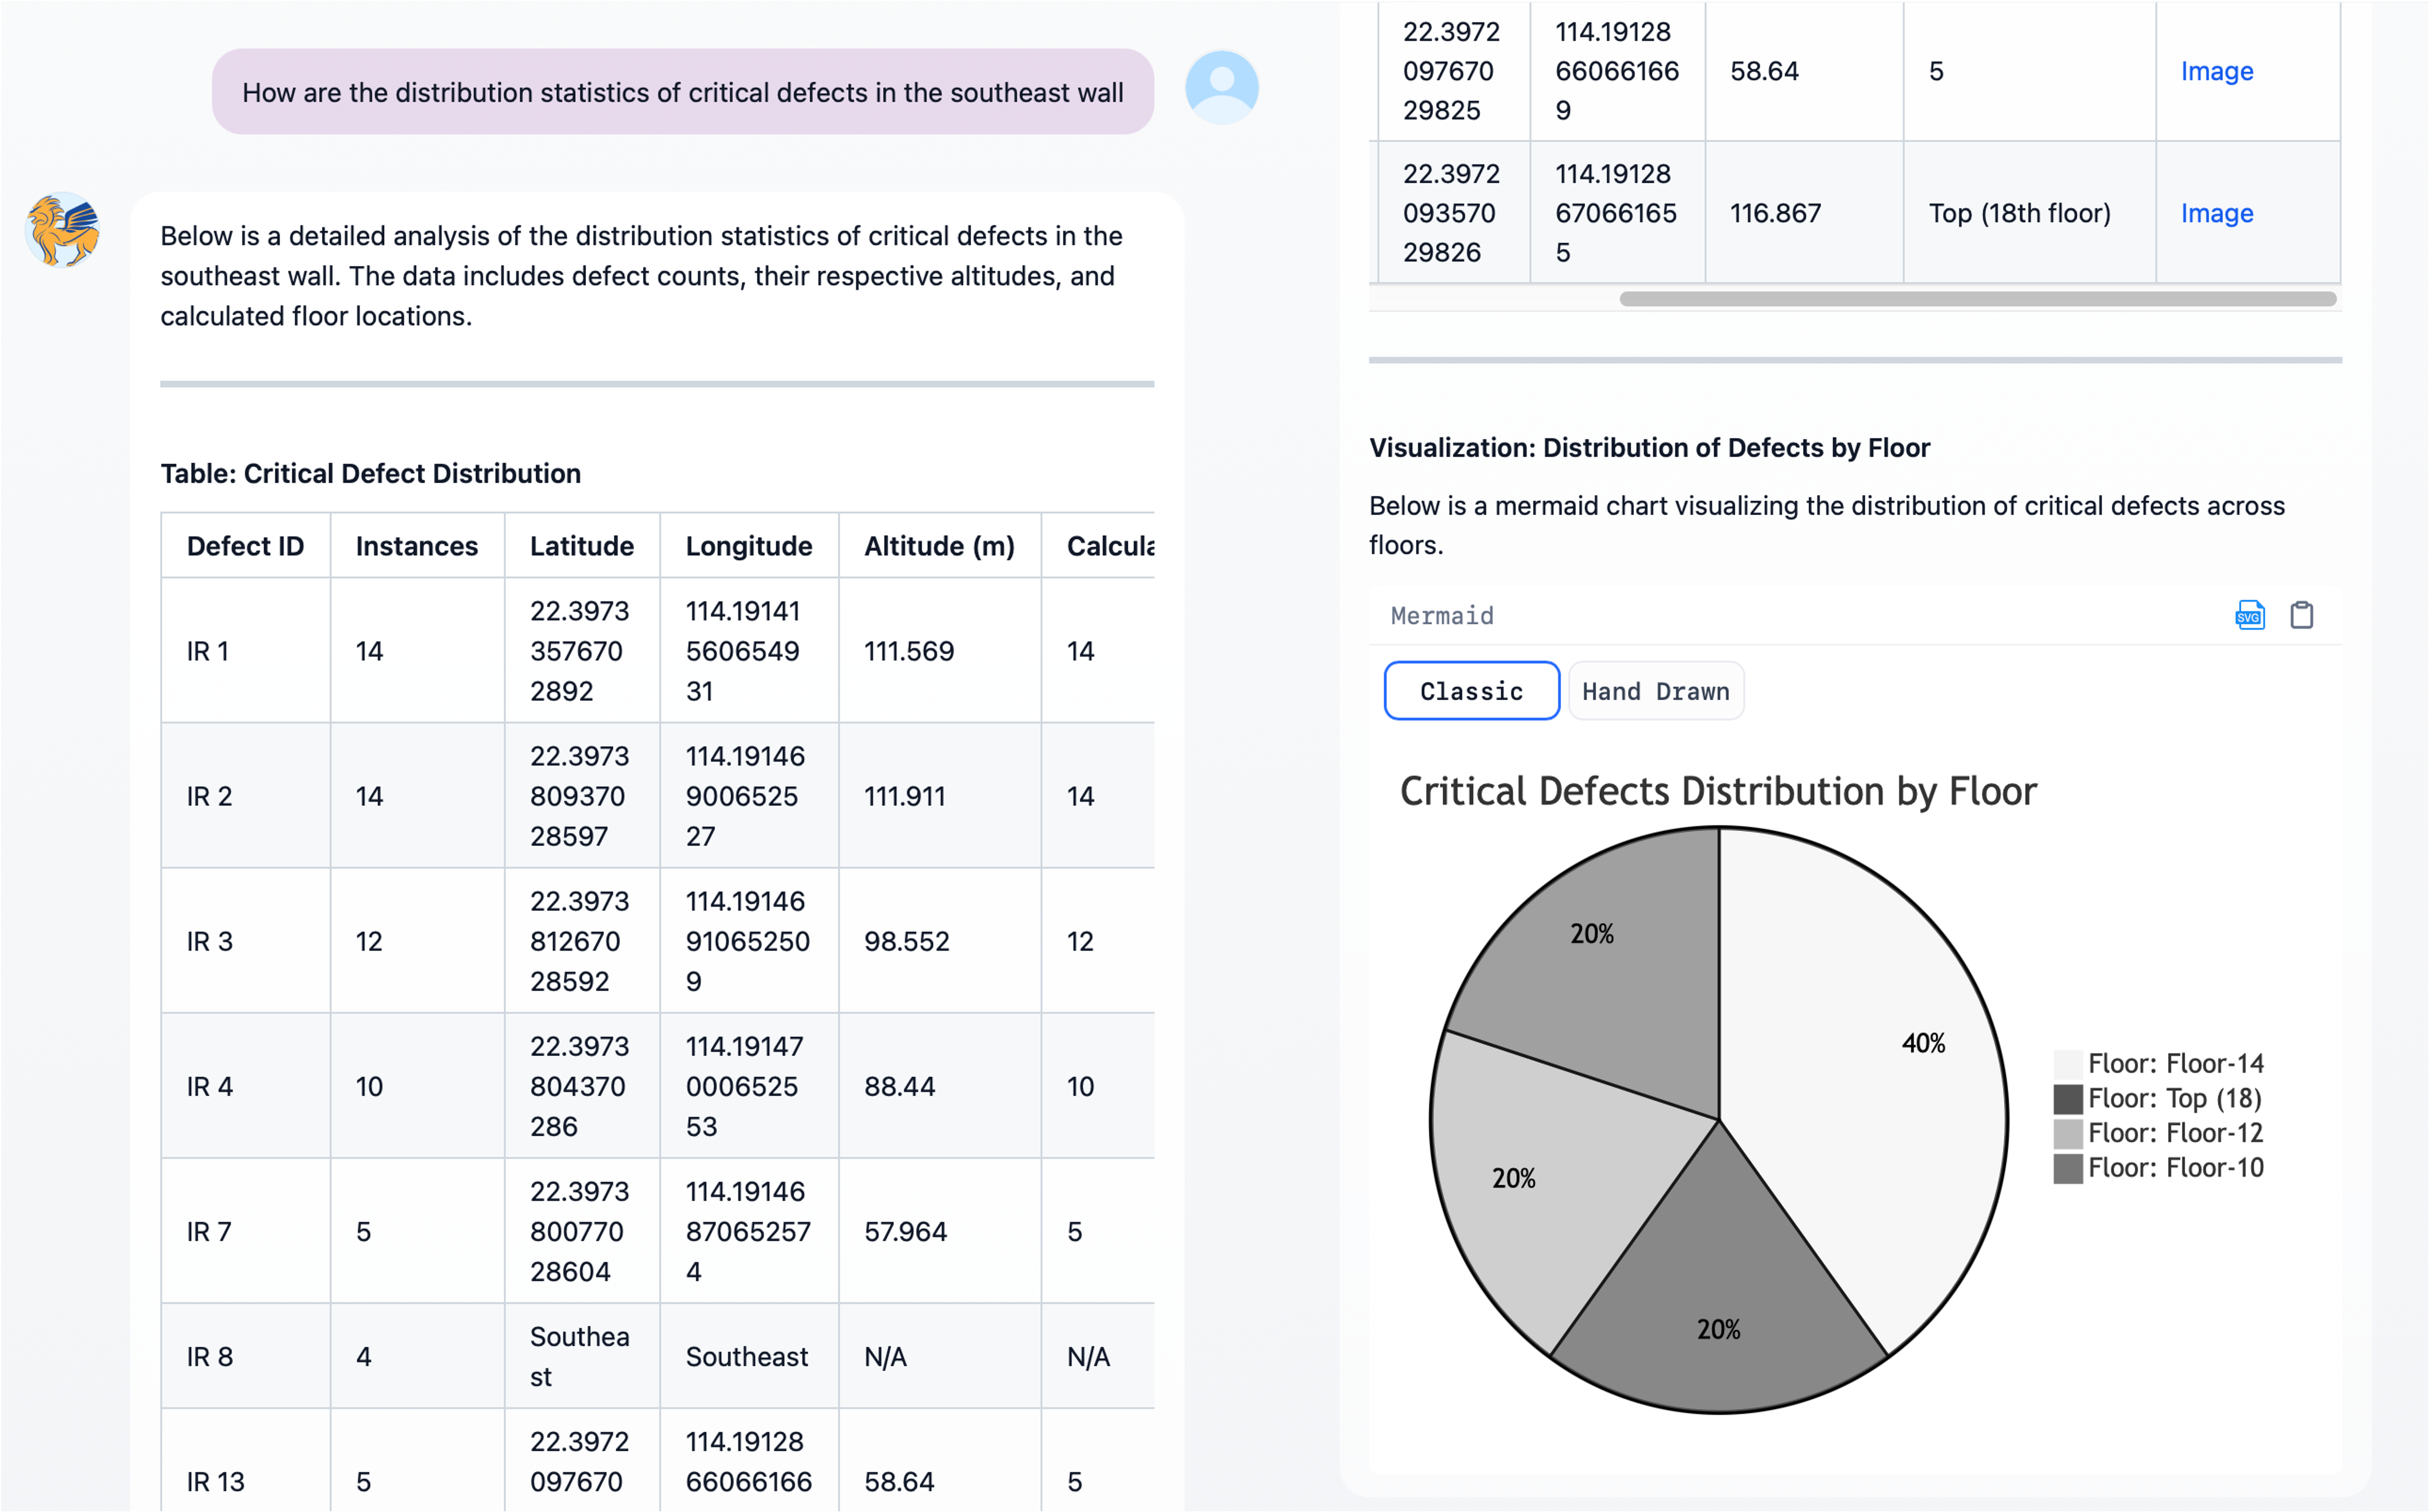
\includegraphics[width=0.6\linewidth]{defectgpt_interface.png}

        \caption{DefectGPT analysis interface demonstrating comprehensive defect distribution analysis capabilities. The system processes natural language queries and automatically generates both detailed statistical summaries and intuitive visualizations, enabling rapid interpretation of complex defect patterns across different structural zones.}
    \label{fig:defectgpt_analysis}
\end{figure}

Unlike the dashboard, which focuses on providing in-depth visual analytics and aggregate reports, the mobile interface prioritizes real-time interactions through an intuitive chatbot. Users can pose questions about specific defects, request comparisons, or obtain actionable insights without requiring prior expertise in defect management. The mobile interface further leverages multimodal capabilities, enabling inspectors to upload images of defects for automated analysis or utilize voice input to streamline interactions. For example, a field inspector could upload a photo of a suspected crack, and the platform would immediately classify the defect type, estimate its severity, and suggest potential remediation strategies based on historical data and predefined thresholds.

\begin{figure}
    \centering
    \includegraphics[width=0.6\textwidth]{defectgpt_mobile.png}
    \caption{DefectGPT Mobile Interface: A simplified interface optimized for real-time question-and-answer interactions. It supports multimodal features, including voice input and defect image analysis, enabling field inspectors to perform quick and accurate assessments.}
    \label{fig:defectgpt_mobile}
\end{figure}

The mobile version complements the desktop dashboard by bridging the gap between on-site inspections and centralized defect analysis. While inspectors in the field benefit from quick, actionable insights via the mobile interface, the desktop platform allows facility managers and engineers to perform deeper trend analyses, review cumulative data, and plan long-term interventions. The synchronization between the two interfaces ensures that all data collected in the field is automatically integrated into the central knowledge base, updating both the defect vector index and the DT visualization in near real-time.

From a deployment perspective, the potential for real-time defect classification and proactive monitoring has become a key value proposition. During pilot studies, inspectors noted a 30\% decrease in combined inspection and documentation time, attributing much of this gain to the platform's immediate retrieval of historical building data, such as previously patched spalls or known seepage zones. As a result, teams could dedicate more effort to remediation measures rather than manual data gathering. These preliminary findings suggest that coupling advanced language models with robust RAG and concurrency mechanisms can meaningfully improve inspection workflows, particularly in large-scale facade assessments.

\subsection{System analysis}

Retrieval performance was quantified by computing precision, recall, and Mean Reciprocal Rank (MRR). Fine-grained adjustments of the top-$k$ parameter and the similarity threshold proved vital to sustain high recall without burdening GPT-4 with irrelevant data segments. Under typical operational loads, retrieval latency remained below 300 milliseconds, validating the efficiency of the underlying FAISS index. Notably, queries centered on cracks—often recognized as early indicators of deeper structural flaws—were particularly instructive. The system excelled at pinpointing records describing crack direction, approximate width, and potential steel reinforcement exposure, and it generated mitigation strategies such as epoxy sealing or polymer injection.

\subsection{Quantitative model comparison}
\label{sec:quantitative-comparison}

In order to compare DefectGPT with other state-of-the-art LLMs on building inspection tasks, we conducted both quantitative and qualitative evaluations. We assessed a range of text-generation and summarization metrics, including ROUGE ($1$, $2$, $L$), BLEU, METEOR, BERTScore, and additional domain-specific measures (e.g., Semantic Similarity, specialized "Sequence" coherence). These metrics capture various aspects of text quality, semantic fidelity, and structural coherence. Below, we provide a detailed overview of the results, accompanied by visualizations to illustrate our findings and a discussion of the system's real-world scalability.

\subsubsection{Overall performance and standardized metrics}

Table~\ref{tab:model-comparison} summarizes the performance of the evaluated models. Standard metrics for text generation (ROUGE, BLEU) and semantic understanding (Semantic Similarity, BERTScore) are reported, alongside additional domain-oriented scores such as Jaccard and Sequence coherence. Notably, DefectGPT demonstrates superior outcomes across nearly all metrics, highlighting its balanced capability in generating coherent, semantically accurate texts.

\begin{table*}[t]
\centering
\setlength{\tabcolsep}{2.75pt}
\caption{Performance Comparison of Different Models on Building Inspection Task}
\label{tab:model-comparison}
\begin{tabular}{l|ccc|ccc|ccc}
\toprule
\multirow{2}{*}{\textbf{Model}} & \multicolumn{3}{c|}{\textit{Text Generation}} & \multicolumn{3}{c|}{\textit{Semantic Understanding}} & \multicolumn{3}{c}{\textit{Additional Metrics}} \\
\cmidrule{2-10}
 & ROUGE-1 & ROUGE-2 & ROUGE-L & BLEU & Semantic & BERTScore & METEOR & Jaccard & Sequence \\
\midrule
GPT-4o & 0.293 & 0.066 & 0.191 & 0.056 & 0.629 & 0.797 & 0.167 & 0.108 & 0.067 \\
Claude-3.5 & 0.292 & 0.046 & 0.184 & 0.020 & 0.591 & 0.798 & 0.114 & 0.078 & 0.063 \\
Mistral-Large & 0.291 & 0.050 & 0.188 & 0.019 & 0.556 & 0.784 & 0.113 & 0.076 & 0.064 \\
Gemini-1.5-Pro & 0.358 & 0.093 & 0.223 & 0.051 & 0.655 & 0.811 & 0.194 & 0.139 & 0.075 \\
Llama-3.1-405B & 0.337 & 0.092 & 0.213 & 0.053 & 0.601 & 0.795 & 0.184 & 0.129 & 0.072 \\
\midrule
\textbf{DefectGPT (Ours)} & \textbf{0.592} & \textbf{0.297} & \textbf{0.503} & \textbf{0.233} & \textbf{0.856} & \textbf{0.905} & \textbf{0.423} & \textbf{0.306} & \textbf{0.273} \\
\bottomrule
\end{tabular}
\end{table*}

To better visualize the relative strengths and weaknesses of the models, we standardized each metric and plotted the results as a heatmap (Fig.~\ref{fig:heatmap}). The vertical axis lists seven models, and the horizontal axis lists eight key metrics. Colors reflect each model's standardized deviation from the mean for that metric: darker shades near +2.0 imply stronger relative performance, whereas lighter shades near -2.0 suggest weaker performance. From the heatmap, DefectGPT (bottom row) exhibits strikingly higher standardized scores in BLEU and METEOR, with near-average performance in ROUGE-1 and ROUGE-L. In contrast, GPT-4o (top row) performs strongly in semantic-related metrics but dips modestly in BLEU.

\begin{figure}[htbp]
    \centering
    % Adjust width as needed, e.g., 0.9\linewidth
    \includegraphics[width=0.8\linewidth]{model_performance_heatmap.png}
    \caption{Model Performance Comparison Heatmap. Rows represent models, columns represent evaluation metrics (ROUGE-1, ROUGE-2, ROUGE-L, BLEU, Semantic Similarity, BERTScore, METEOR, etc.). Colors convey standardized z-scores, with darker shades toward +2.0 indicating better performance.}
    \label{fig:heatmap}
\end{figure}

\subsubsection{Visual score distributions and analysis}

Beyond averages and standardized heatmaps, we also depict the models' performance distributions. Fig.~\ref{fig:radar-plot} provides a radar plot of standardized scores for each model. The radial axes correspond to various metrics, and each polygon's shape illustrates where a particular model excels or lags. Here, DefectGPT (red outline) notably stretches out along the BLEU and METEOR axes, while GPT-4o (dark outline) scores higher on ROUGE-2 but is comparatively narrower in BLEU.

\begin{figure}[htbp]
    \centering
    \includegraphics[width=0.4\linewidth]{performance_radar_plot.png}
    \caption{Standardized Performance Radar Plot. Each axis corresponds to a text-evaluation metric (e.g., ROUGE-1, BLEU, ROUGE-2, ROUGE-L, and METEOR). The distance from the center indicates standardized performance relative to the model averages.}
    \label{fig:radar-plot}
\end{figure}

To further dissect how these metrics vary across different text samples, we employed violin plots (Fig.~\ref{fig:violin-distribution}) for five key metrics (ROUGE-1, ROUGE-2, ROUGE-L, BLEU, METEOR). Each subplot illustrates the distribution of model outputs over an extensive set of building-inspection test data, with the width of each violin signifying the density of scores. Mean performance for each model is marked on the right-hand side of each plot. As shown, DefectGPT's BLEU distribution is skewed towards higher values with lower variance, while GPT-4o exhibits a somewhat broader distribution in ROUGE-2.

\begin{figure}[htbp]
    \centering
    \includegraphics[width=0.85\linewidth]{performance_metrics_distribution.png}
    \caption{Performance Metrics Distribution Analysis using violin plots for each metric. The x-axis in each subplot shows the metric's possible score range, and the y-axis indicates the density. Markers for each model (GPT-4o, Claude 3.5, Mistral-Large-2, Gemini-1.5-Pro, Llama-3.1-405B, DefectGPT) appear on the right side of each violin to indicate average performance.}
    \label{fig:violin-distribution}
\end{figure}

\subsubsection{Scalability, resource utilization, and real-World outcomes}

In addition to these performance metrics, DefectGPT's scalability was rigorously tested under high concurrency scenarios. Stress testing simulated up to 500 concurrent users submitting building inspection queries (e.g., evaluating crack propagation margins or searching for rebar corrosion risks). A specialized concurrency management layer ensured that large-batch embedding requests were processed efficiently without introducing significant queuing bottlenecks, underscoring the system's suitability for broader adoption.

From a deployment perspective, the potential for real-time defect classification and proactive monitoring has become a key value proposition. During pilot studies, inspectors noted a 30\% decrease in combined inspection and documentation time, attributing much of this gain to the platform's immediate retrieval of historical building data, such as previously patched spalls or known seepage zones. As a result, teams could dedicate more effort to remediation measures rather than manual data gathering. These preliminary findings suggest that coupling advanced language models with robust RAG and concurrency mechanisms can meaningfully improve inspection workflows, particularly in large-scale facade assessments.

\section{Discussion}
\label{sec:discussion}

The DefectGPT framework demonstrates several key advantages over traditional building defect management approaches. By integrating DT technology with RAG-enhanced LLMs, our system addresses critical challenges in the building inspection domain that previous methods have struggled to overcome.

\subsection{Innovations in multimodal analysis}

A key innovation of the platform lies in its support for multimodal analysis. By integrating advanced image recognition algorithms and natural language processing models, the mobile interface can process complex user queries that combine text, voice, and images. This enables a more comprehensive understanding of defects, especially in scenarios where textual descriptions alone are insufficient. For instance, an uploaded image of spalling can be cross-referenced with historical data to identify patterns, while a voice query might ask for a detailed explanation of the underlying causes. These capabilities significantly enhance the platform's usability and make it a versatile tool for both technical and non-technical users.

The dual-interface system demonstrates significant practical benefits for defect management workflows. For example, inspectors can identify a critical defect in the field using the mobile interface and flag it for immediate attention, while facility managers simultaneously review aggregated inspection reports on the desktop dashboard to prioritize resources. The integration of multimodal capabilities further enhances efficiency, as users can combine visual, textual, and auditory inputs to interact with the system in a natural and intuitive manner. By combining the strengths of desktop and mobile technologies, the DefectGPT platform delivers a unified solution that is both flexible and robust, addressing the diverse needs of modern building defect management.

\subsection{Performance analysis across different defect types}

Our evaluation reveals varying system performance across different defect types. For crack detection and analysis, the system achieved particularly high accuracy and comprehensive contextual understanding. This is likely due to the extensive documentation of crack-related issues in the training corpus and the visual distinctiveness of cracks in inspection images. In contrast, water seepage detection showed moderate performance, with challenges arising from the temporal nature of these defects and their variable manifestation under different environmental conditions.

The system's performance in detecting and analyzing spalling was notable, with accurate identification of spalling boundaries and robust estimation of affected areas. However, challenges remained in distinguishing between surface-level spalling and deeper structural deterioration, highlighting areas for future improvement in multi-modal sensing integration.

\subsection{Integration challenges and solutions}

The implementation of DefectGPT revealed several integration challenges, particularly in harmonizing data across different sources and formats. Initial difficulties in aligning BIM coordinates with UAV-captured imagery required the development of sophisticated registration algorithms, as detailed in Section 3.1. Similarly, the integration of historical inspection records into a format suitable for vector embedding presented challenges in standardization and semantic normalization.

These challenges were addressed through iterative refinement of the data processing pipeline and the development of custom transformation algorithms. The resulting system demonstrates how these integration obstacles can be effectively overcome, providing valuable insights for future implementations of similar DT-based inspection systems.

\subsection{Comparison with traditional inspection methods}

Beyond the quantitative comparison with other LLM-based systems presented in Section \ref{sec:quantitative-comparison}, our evaluation included a comparative assessment against traditional building inspection methodologies. Compared to conventional paper-based inspection methods, DefectGPT demonstrated a significant reduction in both inspection time and documentation effort. The accuracy of defect identification also improved, with a notable increase in detection rates for minor defects that might be overlooked in traditional visual inspections.

These improvements stem from several factors: the systematic coverage provided by UAV-based image capture, the consistency of automated defect detection algorithms, and the comprehensive retrieval of relevant historical data. The system's ability to correlate current observations with historical patterns also enables more sophisticated trend analysis than is typically possible with manual methods.

\section{Conclusion}

This research developed DefectGPT, an integrated framework that combines digital twin technology with large language models for enhanced building defect management. The system leverages UAV-acquired data, BIM-GIS integration, and advanced RAG-enhanced LLMs to create a comprehensive solution for building inspection and maintenance. Experimental results demonstrate significant improvements in inspection efficiency and defect detection rates compared to traditional methods. The multimodal analysis capabilities enable users to process complex queries combining text, images, and voice inputs, while the context-aware retrieval system provides highly relevant historical information to support decision-making. The integration of domain-specific knowledge with advanced language models creates a powerful tool for building professionals, enhancing their ability to identify, analyze, and manage structural defects throughout a building's lifecycle. By addressing the limitations of conventional inspection approaches, DefectGPT represents a significant advancement in intelligent infrastructure management and provides a solid foundation for future developments in automated building maintenance systems.

\section{Declaration of Competing Interest}

The authors confirm that they have mentioned all organizations that funded this research in the Acknowledgements section of the submission, including grant numbers where appropriate. The authors declare that they have no commercial or associative interest that represents a conflict of interest with other people or organizations that can inappropriately influence their work.


\section{Acknowledgements}

This study was supported in part by the InnoHK initiative of the Innovation and Technology Commission of the Hong Kong Special Administrative Region Government via the Hong Kong Centre for Logistics Robotics (Grant Nos: 14217922, 14209623, 14209424 and 14200524).

\printcredits

%% Loading bibliography style file
%\bibliographystyle{model1-num-names}
%\bibliographystyle{cas-model2-names.bst}
\bibliographystyle{unsrt}
% Loading bibliography database
\bibliography{defectAgent}
% Biography
%\bio{}
% Here goes the biography details.
%\endbio

%\bio{pic1}
% Here goes the biography details.
%\endbio


\end{document}
